\documentclass[12pt]{scrreprt}
\usepackage[T1]{fontenc}
\usepackage[finnish]{babel}
\usepackage[utf8]{inputenc}
\usepackage{amsmath}
\usepackage[toc,page]{appendix}
\usepackage[pdftex]{graphicx}
\usepackage{hyperref}

\renewcommand\emph{\textbf}
\addto\captionsfinnish{
  \renewcommand{\bibname}{Lähteet}
  \renewcommand{\appendixname}{Liitteet}
  \renewcommand{\appendixpagename}{Liitteet}
}
\renewcommand\appendixtocname{Liitteet}
\linespread{1.3}

\title{Mulla on nälkä!}
\subtitle{Maatalouden tuotanto Somaliassa sääolosuhteiden funktiona}
\author{Jaakko Hannikainen \and Cliona Shakespeare}
\date{\today}
\publishers{Valkeakosken Tietotien lukio / Päivölän Kansanopisto\\
            Tieteenala: Mallintaminen}
\begin{document}
  \maketitle

  \begin{abstract}
    Climate change will have a definite impact on humanitarian aid. To find out how climate change would affect aid, a What If? Network was created to generate results by data farming. Our responsibility was the agriculture model.
The model takes data on the week's average temperature, cumulative rainfall and sunlight, and the soil's acidity, then transforms these into coefficients, from which a weekly coefficient is made using the following formula:
  \begin{em}
  $ \text{viikkokerroin} = (\text{vesikerroin}) \times (\text{lämpökerroin})
  \times (\text{valokerroin}) \times (\text{pHkerroin}) $\end{em}

The total crop yield is calculated using the following formula:
  \begin{em}
  $ \text{sato} = (\text{pinta-ala}) \times (\text{teoreettinen maksimisato per
  alueyksikko}) \times (\text{viikkokerrointen keskiarvo}) $\end{em}

Each crop has its own coefficient conversion formulae.
We have also simulated the milk production of cows:
\begin{em}
  $ \text{maidon määrä (kg)} = 0.3375 \times \text{ruoan määrä (kg)}
  + 8.325\text{kg} $ \end{em}

(results)
  \end{abstract}

  \tableofcontents

  \chapter{Johdanto}

  % Mitä: Somalia on kehitysmaa, ongelmia: ruokaa ei ole tarpeeksi jne,
  % ongelmien mallintamiseksi tämä simulaatio
  
  Maailman kriisialueilla avustusjärjestöt haluavat tietää, miten ne saisivat 
  autettua ihmisiä mahdollisimman tehokkaasti rajatuilla resursseilla. Tätä 
  varten olemme osallistuneet mallintamisprojektiin \cite{scythe}, jossa mallinnetaan
  ilmastonmuutoksen vaikutusta humanitääriseen avustukseen. Tämän osaprojektin aiheena on maatalous. Ruoan tuotantoon ja kulutukseen liittyvät ilmasto-, vesi-, logistiikka- ja karttamallit. [gameon-viite]
Esimerkkitapauksemme Somalia on afrikkalainen kehitysmaa, jolla ei ole ollut 1990-luvun jälkeen toimivaa hallitusta. Yksi sen lukuisista ongelmista on se, että ruokaa ei ole tarpeeksi kaikille, mikä johtaan nälänhätään, kulkutautien leviämiseen, ja ihmisten kuolemiseen. 
Tutkimuskysymyksemme on, kuinka paljon ruokaa pelloilta tulee tietyissä olosuhteissa.
Dataviljely?

  \includegraphics[width=10cm]{projectmap.png}
  
  % Ruokaa ei tarpeeksi → nälänhätä → kulkutauteja → ihmisiä kuolee → Ongelma.
  
  % Miksi ei karjataloutta tms
  
  % Miksi: tulevaisuuden mallintaminen ja ennustaminen (Somalia! Suomen
  % nälkävuodet!), humanitaarisen avustuksen vaikutukset, ihmiskärsimyksen
  % vähentäminen 
  
  % Ilmiön idea (Somaliassa kasvatetaan ruokaa. Tätä pitää mallintaa.)
  
  % tulevaisuuden ennustaminen on kivaa – miksi?
  
  \chapter{Aineisto ja menetelmät}
  
  \section{Dataviljely}
  
  Dataviljely on menetelmä, joka perustuu siihen, että mahdollisimman yksinkertaista
  mallia ajetaan mahdollisimman monta kertaa. Tästä tulee jakauma tuloksia, joiden
  analyysillä voidaan vetää johtopäätöksiä mallinnetusta ilmiöstä. \cite{assimple}
  Rapid scenario prototyping on tärkeä osa dataviljelyä. Siinä luotua mallia ajetaan
  yksillä parametreillä testitilanteessa, siten, että sitä aina parannetaan saaujen
  tulosten perusteella. [viite asd]

  \section{Ilmiö}

  Maatalous on järjestelmällistä kasvien tai karjan kasvattamista suurella mittakaavalla ihmistarpeeseen. Maanviljely on kasvien, esimerkiksi viljojen, kasvattamista.
  % maatalous yleisesti ^
Osana tutkimusprojektikokonaisuutta Roosa Räty tutki, mitä Somaliassa syödään ja kasvatetaan.  Käytimme hänen tuloksiaan valitessamme kasvilajikkeita tutkittavaksi. Lisäksi saimme tietää, että vaikka Somaliassa juodaan paljon maitoa, naudanlihaa ei syödä. [Räty]

Kasvien kasvamiseen vaikuttavista tekijöistä olemme ottaneet huomioon sääolosuhteet (sadanta, lämpötila, auringonvalon määrä) ja maaperän pH:n. Olemme jättäneet huomiotta muun muassa lehtien pinta-alan, haihtumisen, juurien tiheyden, leveyspiirin ja tuulen vaikutukset satoon.

Lisäksi olemme huomioineet, että tulvat aiheuttavat satojen tuhoutumisen. Kuivuus on otettu huomioon sadannassa, ja joulukuusta helmikuuhun mikään ei kasva, koska on liian kuivaa.
  
  \section{Malli}

  Kun sadon määrää simuloidaan, käytetyt parametrit ovat sademäärä, lämpötila, auringonvalon määrä ja maaperän pH. Jokaisella on optimiarvo, jolla saadaan maksimisato. Mitä enemmän optimialueelta poiketaan, sitä enemmän sadon määrä laskee. Poikkeuksena on auringonvalo, jossa sadon määrä ei laske, jos auringonvaloa saadaan yli optimin.

  \begin{em}
  $ \text{sato} = (\text{pinta-ala}) \times (\text{teoreettinen maksimisato per
  alueyksikko}) \times (\text{viikkokerrointen keskiarvo}) $\end{em}
  jossa jokainen viikkokerroin saadaan kaavalla

  \begin{em}
  $ \text{viikkokerroin} = (\text{vesikerroin}) \times (\text{lämpökerroin})
  \times (\text{valokerroin}) \times (\text{pHkerroin}) $\end{em}
  
  Kertoimet lasketaan kaavoilla:
  0, jos x ≥  yläarvo tai x ≤ ala-arvo.
  kx+b, jos ala-arvo < x < optimi tai optimi < x < yläarvo
  1, jos x = optimi.
  Auringonvaloille kertoimet lasketaan:
  0, jos x ≤ ala-arvo
  kx+b, jos ala-arvo < x < optimi
  1, jos x ≥ optimi.
  
  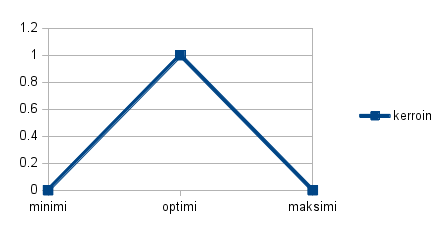
\includegraphics[width=10cm]{coefficientgraph.png}

  % funktioiden kuvaus

  % Lyhyt kuvaus jokaisesta mahdollisesta viljelyskasvista; maissi, vehnä, durra

  % Perustelut juuri näille parametreille, kuvaus parametreistä, kuvaus,
  % merkitys, mahdolliset arvot, yksikkö → teoreettiset minimi- ja maksimiarvot
  % sadolle

  \subsection{Viljelykasvit}

  Koska eri kasvit kasvavat optimaalisesti hyvinkin eri olosuhteissa, kerromme tässä arvoista, joita käytämme mallissamme parametrien oletusarvoina. Maissi ja vehnä ovat tarkastelussa mukana sen takia, että ne ovat yleisiä viljelyskasveja, durra on Afrikan ja Aasian kuivilla alueilla esiintyvä viljelyskasvi.  
  
  Maissi on kasvi, joka tuottaa yleensä keltaisia siemeniä. Siemenet ovat
  syötävä osa, loput kasvista jätetään syömättä. Maissi tarvitsee kostean ja
  ravinteikkaan maaperän. Sille ideaali vesimäärä olisi \cite{cropwater} mukaan
  keskimäärin 0.29 cm/vrk; annoimme parametrillemme vaihteluvälin 0.145 cm/vrk
  – 0.425 cm/vrk. \cite{ugandamaize} ja \cite{plessismaize} antavat maissille
  eri kasvulämpötiloja (5$^{\circ}$C – 42$^{\circ}$C ja 10$^{\circ}$C –
  32$^{\circ}$C). Mallinnuksen helpottamiseksi olemme valinneet
  lämpötilajakaumaksi 20$^{\circ}$C – 40$^{\circ}$C, optimi 30$^{\circ}$C.
  Maissille sopiva pH on välillä 5.5 – 7.0 \cite{corngrowing}. Käytämme
  ideaalina näiden keskiarvoa 6.25. Auringonvalolle arvioimme optimiksi
  8h/päivä, minimi 6 tuntia päivässä. Maissi kasvaa 18 viikossa.
  Maksimiarvomme sadolle on 8 tonnia hehtaaria kohden \cite{iita}.

  Vehnä on Suomessakin kasvava vilja. Sille ideaalilämpötila olisi 19$^{\circ}$C
  - 25$^{\circ}$C \cite{wheat}, valitsimme optimiksemme 22$^{\circ}$C. Käytämme
  pH:n jakaumana 6-7:ää \cite{wheatfert}, optimi 6,5. Veden ideaalimäärä olisi
  0.31 cm/vrk \cite{cropwater}, jakauma  0.155 – 0.465 cm/vrk. \cite{growwheat}
  mukaan vehnä tarvitsisi noin 6 tuntia auringonvaloa päivässä, minimi 4 tuntia 
  päivässä. Vehnä kasvaa noin 15 viikossa. Vehnää tulee maksimiarvona noin 8 tonnia 
  hehtaaria kohden \cite{sri}.

  Durra on viljalaji, joko kasvaa trooppisissa ja subtrooppisissa ilmastoissa.
  Sen vedentarve on noin 0.38 cm/vrk \cite{cropwater}, jakauma 0.19 –
  0.57 cm/vrk. Durran ideaalilämpötila on 20-40$^{\circ}$C [10], optimina
  käytimme näiden keskiarvoa 30$^{\circ}$C. Sille ideaali pH-jakauma olisi 5-8.5
  \cite{moench}, käytämme optimina keskiarvoa 6.75. Auringonvalolle arvioimme
  optimiksi 8h/päivä, minimi 6 tuntia päivässä. Durra kasvaa noin 18
  viikossa. Sen teoreettinen maksimisato on 3 tonnia / hehtaari \cite{wylie}.

  \subsection{Maidon tuotanto}
  450-kiloinen lehmä tuottaa \cite{milk} mukaan maitoa kaavalla
  
  \begin{em}
  $ \text{maidon määrä (kg)} = 0.3375 \times \text{ruoan määrä (kg)}
  + 8.325\text{kg} $ \end{em}

  Arvioimme, että hehtaarille mahtuisi noin kymmenen lehmää. Mallissamme lehmien
  määrä lisääntyy kahdella prosentilla vuosittain. Maidon tuotanto lasketaan
  kokonaisista lehmistä, eli jos lehmiä olisi 2.63, maitoa tulisi kahden lehmän
  verran.

  \chapter{Tulos}

  \section{Mallin käyttö simulaatiossa}

  Päätimme varioida maisssin ja durran kasvun optimilämpötiloja ja -vesimääriä. Tällä pystyimme simuloimaan erilaisten lajikkeiden vaikutusta Somalian oloihin. Koesuunnittelun teki Mirjam Kauppila.

  Vaihteluväli lämpötilan optimille oli molemmissa tapauksissa 30-40$^{\circ}$C,
  siten että lämpötilajaauman ääriarvot olivat 10$^{\circ}$ päässä optimista.
  Maissille vesimäärän optimin vaihteluväli oli 1.5-3 cm/vk, durralle
  2-3.5cm/vk. Veden minimi oli 0.5 $\times$ optimi ja maksimi oli 1.5 $\times$
  optimi.

  koodi

  malli to koodiprosessi + koodin kuvailu

  \section{Testiajot}

  kauniita kuvia

  \chapter{Johtopäätökset}

  saimme xyz tulokset, järkevyys? mielenkiintoisuus? mallin kehitys? käyttökelpoisuus? käytettävyys?
  
malli hyvä, koska

paitsi että täyttä kuraa (kesken, yksinkertaistettu), asiat A-Ö, 1-9 ja loputkin huonosti parametroitu tai jätetty huomiotta jne; karjatalous! tarvitsee enemmän/parempaa lähtödataa

siitä huolimatta: auttaa ymmärtämistä, osa kokonaisuutta, toimii ihan OK

Esimerkki mallin käytöstä: avustusjärjestö haluaa tietää, miten se saisi autettua ihmisiä mahdollisimman tehokkaasti rajatuilla resursseilla. Järjestö pyörittää simulaatiota usein alkuarvoin, ja katsoo, millaisia tuloksia tulee milläkin alkuarvoilla. Järjestö voi käyttää näitä tietoja hyväkseen päätöksenteossaan.

  \begin{thebibliography}{9}
  
  	\bibitem{scythe}
  	Ted Meyer, Merikki Lappi et al.
  	\emph{Climate Change and Humanitarian Assistance: challenges and complications}.
  	
  	\bibitem{assimple}
  	Paul J. Sánchez.
  	\emph{As Simple as Possible, but no Simpler: a Gentle Introduction to Simulation Modeling}

    \bibitem{cropwater}
    Wright \& Killer.
    \emph{Average water use for multiple crops}.
    2002.
    Haettu \today. \\
    \url{http://www.extension.umn.edu/distribution/cropsystems/components/DC1322a.pdf}

    \bibitem{ugandamaize}
    Ministry of Agriculture, Uganda.
    \emph{Maize production}.

    \bibitem{plessismaize}
    Jéan du Plessis.
    \emph{Maize production}.
    Haettu \today. \\
    \url{http://www.arc.agric.za/arc-gci/Fact%20Sheets%20Library/Maize-infopak.pdf}

    \bibitem{iita}
    IITA.
    \emph{Research to Nourish Africa, Maize}.
    Haettu \today. \\
    \url{http://old.iita.org/cms/details/maize_project_details.aspx?zoneid=63&articleid=273}

    \bibitem{sri}
    Joku.
    \emph{Cultivating Wheat With SRI}.
    Joskus.
    Jossakin.

    \bibitem{corngrowing}
    Joku.
    \emph{Corn Growing and Harvest Information}.
    Haettu \today. \\
    \url{http://veggieharvest.com/vegetables/corn.html}

    \bibitem{wheat}
    Exploring the Environment Team.
    \emph{Wheat}.
    Haettu \today. \\
    \url{http://www.cotf.edu/ete/modules/climate/GCwheat3.html}

    \bibitem{wheatfert}
    M. L. Vitosh.
    \emph{Wheat Fertility and Fertilization}.

    \bibitem{growwheat}
    GrowingAnything.com.
    \emph{How to Grow Wheat}.
    Haettu \today. \\
    \url{http://www.growinganything.com/how-to-grow-wheat.html}
        
    \bibitem{peacock}
    J. M. Peacock.
    \emph{Response and Tolerance of Sorghum to Temperature Stress}.
    Joskus.

    \bibitem{moench}
    Food and Agriculture Organisation.
    \emph{Sorghum bicolor (L) Moench}.
    Haettu \today. \\
    \url{http://www.fao.org/ag/agp/agpc/doc/gbase/data/pf000319.htm}

    \bibitem{wylie}
    Peter Wylie.
    \emph{Managing sorghum for high yields}.
    Joskus.

    \bibitem{milk}
    Beth Wheeler.
    \emph{Guidlines to Feeding Dairy Cows}.
    Haettu \today.
    \url{http://en.engormix.com/MA-dairy-cattle/management/articles/guidelines-feeding-dairy-cows-t49/124-p0.htm}

  \end{thebibliography}

  \begin{appendices}

  \chapter{Ohjelmakoodi}
  
  \section{Juttu.java}
  
  Java-koodia.
  
  \section{ToinenJuttu.java}

  Lisää Javaa.

  \chapter{Data $\rightarrow$ kerroin}
   
  ...?

  \end{appendices}

\end{document}
